% Template for ICASSP-2026 paper; to be used with:
%          spconf.sty  - ICASSP/ICIP LaTeX style file, and
%          IEEEbib.bst - IEEE bibliography style file.
% --------------------------------------------------------------------------
\documentclass{article}
\usepackage{spconf,amsmath,graphicx,hyperref}
\usepackage{xspace}
\usepackage{booktabs}
\usepackage[table]{xcolor}

% Example definitions.
% --------------------
\def\x{{\mathbf x}}
\def\L{{\cal L}}
\newcommand{\ourmethod}{{\fontfamily{lmtt}\selectfont \textbf{TTARAG}}\xspace}
\DeclareMathOperator*{\argmax}{arg\,max}

% Title.
% ------
\title{Predict the Retrieval! Test Time Adaptation for Retrieval Augmented Generation}
%
% Single address.
% ---------------

\name{Xin Sun$^{1}$ Zhongqi Chen$^{2}$ Qiang Liu$^{1}$ Shu Wu$^{1}$ Bowen Song$^{2}$ Weiqiang Wang$^{2}$ Zilei Wang$^{3}$ Liang Wang$^{1}$}
\address{$^{1}$ NLPR, MAIS, CASIA $^{2}$ Ant Group $^{3}$ USTC\\ xin.sun@cripic.ia.ac.cn,  \{qiang.liu, shu.wu, wangliang\}@nlpr.ia.ac.cn, zlwang@ustc.edu.cn, \\
 \{chenzhongqi.czq, bowen.sbw, weiqiang.wwq\}@antgroup.com}
%
% For example:
% ------------
%\address{School\\
%	Department\\
%	Address}
%
% Two addresses (uncomment and modify for two-address case).
% ----------------------------------------------------------
%\twoauthors
%  {A. Author-one, B. Author-two\sthanks{Thanks to XYZ agency for funding.}}
%	{School A-B\\
%	Department A-B\\
%	Address A-B}
%  {C. Author-three, D. Author-four\sthanks{The fourth author performed the work
%	while at ...}}
%	{School C-D\\
%	Department C-D\\
%	Address C-D}
%
\begin{document}
\ninept
%
\maketitle
%
\begin{abstract}
Retrieval-Augmented Generation (RAG) has emerged as a powerful approach for enhancing large language models' question-answering capabilities through the integration of external knowledge. However, when adapting RAG systems to specialized domains, challenges arise from distribution shifts, resulting in suboptimal generalization performance. In this work, we propose \ourmethod, a test-time adaptation method that dynamically updates the language model's parameters during inference to improve RAG system performance in specialized domains. Our method introduces a simple yet effective approach where the model learns to predict retrieved content, enabling automatic parameter adjustment to the target domain. Through extensive experiments across six specialized domains, we demonstrate that \ourmethod achieves substantial performance improvements over baseline RAG systems. Code available at \url{https://github.com/sunxin000/TTARAG}.
\end{abstract}
%
\begin{keywords}
Retrieval Augmented Generation, Test-Time Adaptation, Self-Supervised Learning, Domain Adaptation
\end{keywords}
%
\section{Introduction}
Retrieval-Augmented Generation (RAG) \cite{izacard2021leveraging, lewis2020retrieval, edge2024local} has emerged as a crucial approach for enhancing large language models (LLMs) \cite{radford2019language, brown2020language, bubeck2023sparks} by addressing their inherent knowledge limitations. Through the integration of external knowledge sources \cite{pasca-2019-wikipedia, bollacker2008freebase, jin2019pubmedqa}, RAG systems not only improve the accuracy of LLM responses but also help mitigate hallucination issues while eliminating the need for extensive model retraining.

However, while most current research has focused on the effectiveness of RAG systems for general domains, significant challenges persist in adapting these systems to specialized domains. These systems often struggle with distribution shifts and domain-specific data dependencies \cite{xu2025simragselfimprovingretrievalaugmentedgeneration, shi2024medadapter}, frequently failing to accurately utilize information in domain-specific contexts \cite{miller2020effect, liu-etal-2022-challenges}. 

To address these challenges, test-time adaptation (TTA) \cite{sun2020test, karmanov2024efficienttesttimeadaptationvisionlanguage} offers a promising solution. TTA allows models to dynamically adjust their parameters at inference time, typically through self-supervised learning objectives derived from the test data itself, without requiring new labeled data \cite{liang2024comprehensive}. This characteristic makes TTA particularly well-suited for scenarios involving domain shifts or distribution changes not seen during initial training, as it enables the model to rapidly specialize to the immediate context. Building on these insights, we propose a simple yet powerful method for adapting RAG systems during inference: \ourmethod. Our approach generates self-supervised learning signals by dividing retrieved passages into prefix-suffix pairs and training the model to predict suffix content from prefix context. This technique enables LLMs to perform real-time parameter updates when encountering new domains, effectively leveraging domain knowledge stored within the model parameters.


Through extensive experiments across six specialized domains, we demonstrate that \ourmethod achieves substantial performance improvements over baseline RAG systems. Our approach consistently outperforms both standard RAG and  baselines like Chain-of-Thought and In-Context Learning, achieving the best results in 19 out of 24 experimental settings while maintaining computational efficiency. These results validate the effectiveness of our approach for domain-specific applications.

\section{Related Work}

\subsection{Retrieval Augmented Generation}
Retrieval Augmented Generation (RAG) \cite{lewis2020retrieval} has emerged as a powerful paradigm for enhancing large language models (LLMs) with external knowledge. By integrating a retrieval system with LLMs, RAG enables models to access and leverage external knowledge sources during generation, effectively addressing the limitations of static, parameterized knowledge in LLMs.

Recent advances in RAG have focused on several key directions. First, researchers have explored dynamic retrieval processes \cite{jiang-etal-2023-active,jeong-etal-2024-adaptive} to improve the relevance of retrieved content. Second, various filtering mechanisms \cite{robustlm,yu2024rankrag} have been developed to eliminate irrelevant contexts and enhance RAG robustness. Additionally, instruction-tuning methods \cite{liu2024chatqa,lin2024radit} have been specifically designed to improve LLMs' search and RAG capabilities.
\subsection{Test-time inference adaptation}

Test-time inference adaptation aims to adapt pre-trained models to unlabeled test data during inference time without accessing the source training data. This paradigm has gained increasing attention as a practical solution for handling distribution shifts in real-world applications \cite{wang2021tent, boudiaf2022parameter}. Unlike traditional domain adaptation methods that require simultaneous access to both source and target domains, test-time adaptation only needs the pre-trained model and target data, making it more privacy-friendly and storage-efficient \cite{liang2020we}.

Early works in this direction focused on hypothesis transfer learning \cite{kuzborskij2013stability}, where models trained on source domains are adapted to target domains with limited labeled data. Recent advances have extended this to fully unsupervised scenarios, leveraging techniques like entropy minimization \cite{wang2021tent}, self-training \cite{sun2020test}, and test-time normalization statistics calibration \cite{schneider2020improving} to adapt models using only unlabeled test samples. 

Building on these advances, \ourmethod introduces a simple yet effective approach for test-time adaptation in retrieval-augmented generation. By learning to predict subsequent tokens in retrieved passages, \textbf{\ourmethod enables fully unsupervised adaptation without requiring access to source domain data or labeled examples.}



\section{Methodology}
Our approach introduces a test-time adaptation mechanism for retrieval-augmented generation that enables model optimization during inference without access to ground truth labels. The key innovation lies in designing a self-supervised learning objective using retrieved passages as supervision signals. We hypothesize that by training the model to predict a suffix of a passage given its prefix and the original query, the model is encouraged to better understand the contextual relationships and domain-specific language patterns within the retrieved documents. This task inherently pushes the model to learn how information flows and connects within relevant texts, thereby aligning its internal representations more closely with the nuances of the target domain encountered at test time.

\subsection{Overview}
Given a test input query $q$ and retrieved passages $\{p_1, ..., p_k\}$, we formulate a self-supervised adaptation objective by splitting passages into prefix-suffix pairs for prediction:
\begin{equation}
    \mathcal{L}_{adapt} = -\sum_{i=1}^k \log P(p_i^{suffix}|p_i^{prefix}, q; \theta)
\end{equation}
where $\theta$ represents the model parameters.

\begin{figure}[h]
    \centering
    
\includegraphics[width=1.0\linewidth]{framework.pdf}
    \caption{Comparison between Standard RAG and TTARAG systems.}
    \label{fig:overview}
\end{figure}

\iffalse
\begin{figure*}[t]
\centering
\begin{tikzpicture}[
    box/.style={rectangle, draw, thick, minimum height=1cm, minimum width=2.8cm, align=center, font=\small},
    query/.style={box, fill=green!20},
    retriever/.style={box, fill=blue!20},
    passages/.style={box, fill=orange!20},
    llm/.style={box, fill=purple!20},
    answer/.style={box, fill=gray!20},
    tta/.style={box, fill=yellow!20, minimum width=2.5cm},
    adapted/.style={box, fill=green!40},
    arrow/.style={->, thick, >=stealth}
]

% Standard RAG System (Left)
\node[font=\large\bfseries] at (-1.5, 5.5) {Standard RAG System};

\node[query] (q1) at (0, 4.5) {Query};
\node[retriever] (r1) at (0, 3) {Retriever};
\node[passages] (p1) at (0, 1.5) {Passages};
\node[llm] (llm1) at (0, 0) {LLM};
\node[answer] (a1) at (0, -1.5) {Answer};

% Standard RAG arrows
\draw[arrow] (q1) -- (r1);
\draw[arrow] (r1) -- (p1);
\draw[arrow] (p1) -- (llm1);
\draw[arrow] (q1) to[out=180,in=180,looseness=2] (llm1);
\draw[arrow] (llm1) -- (a1);

% TTARAG System (Right)
\node[font=\large\bfseries] at (8.5, 5.5) {TTARAG System};

\node[query] (q2) at (10, 4.5) {Query};
\node[retriever] (r2) at (10, 3) {Retriever};
\node[passages] (p2) at (10, 1.5) {Passages};

% Test-Time Adaptation Module background
\begin{scope}[on background layer]
\node[draw, thick, dashed, rounded corners=5pt, fill=red!10, minimum width=6.5cm, minimum height=2.8cm] at (7, 0.2) {};
\end{scope}
\node[font=\bfseries] at (7, 1.8) {Test-Time Adaptation};

% TTA components
\node[tta] (ps) at (5.2, 0.8) {Passage Splitting\\(Prefix | Suffix)};
\node[tta] (ssl) at (8.8, 0.8) {Self-Supervised\\Learning};
\node[tta] (pu) at (7, -0.5) {Parameter Update\\$\theta \rightarrow \theta'$};

\node[adapted] (llm2) at (10, -1.8) {Adapted LLM};
\node[adapted] (a2) at (10, -3.3) {Enhanced Answer};

% TTARAG arrows
\draw[arrow] (q2) -- (r2);
\draw[arrow] (r2) -- (p2);
\draw[arrow] (p2) -- (ps);
\draw[arrow] (ps) -- (ssl);
\draw[arrow] (ssl) -- (pu);
\draw[arrow] (pu) -- (llm2);
\draw[arrow] (q2) to[out=0,in=0,looseness=2.5] (llm2);
\draw[arrow] (p2) to[out=0,in=90,looseness=0.8] (llm2);
\draw[arrow] (llm2) -- (a2);

\end{tikzpicture}

\caption{Comparison between Standard RAG and TTARAG systems. While standard RAG directly uses retrieved passages for generation, TTARAG introduces a test-time adaptation module that splits passages into prefix-suffix pairs, performs self-supervised learning to predict suffixes from prefixes, and updates model parameters to better align with the target domain before generating the final answer.}
\label{fig:rag_comparison}
\end{figure*} \fi

\subsection{Context Processing}
The adaptation process begins with careful processing of the retrieved passages to create meaningful prefix-suffix pairs for training. 

\noindent\textbf{Length Filtering.} To ensure sufficient context for meaningful adaptation, passages shorter than a configured minimum length threshold are filtered out.

\noindent\textbf{Passage Splitting.} Each passage is split into prefix-suffix pairs using a two-tier strategy:
    \begin{itemize}
        \item \textbf{Primary Strategy} Passages are split at first natural linguistic boundaries marked by punctuation (periods, commas, semicolons, colons, exclamation marks, and question marks)
        \item \textbf{Fallback Strategy} When no suitable punctuation-based split exists, the passage is divided at its midpoint, ensuring each segment contains at least three words.
    \end{itemize}

\subsection{Parameter Adaptation Process}

\subsubsection{Initialization}
Prior to the adaptation process, the model parameters are reset to their original pre-trained state to ensure a clean starting point for each adaptation iteration. 

% An AdamW optimizer is then initialized with carefully configured hyperparameters: learning rate $\alpha$ for controlling update step sizes, epsilon $\epsilon$ for numerical stability, and weight decay $\lambda$ for regularization.

\subsubsection{Training Loop}
For each batch of prefix-suffix pairs:
\begin{equation}
    \theta_t = \theta_{t-1} - \alpha \cdot \frac{1}{N} \sum_{i=1}^N \nabla_\theta \mathcal{L}_{adapt}^i
\end{equation}
where $N$ is the gradient accumulation steps and $\mathcal{L}_{adapt}^i$ is the loss for the $i$-th pair.

During training, the complete text (prefix and suffix) is first tokenized. The model then computes the loss on the suffix prediction task, where prefix tokens are masked during label preparation. To ensure stable training, gradients are accumulated over two steps and clipped to a maximum norm threshold. The AdamW optimizer then updates model parameters using these accumulated gradients. Since we only adapt on 3 prefix-suffix pairs in our experiments, the computational overhead remains acceptable.



\subsection{Response Generation}
After parameter adaptation, the model generates the final response using the adapted parameters $\theta'$:
\begin{equation}
    y = \argmax_y P(y|q, \{p_1, ..., p_k\}; \theta')
\end{equation}

% This approach enables effective domain adaptation through self-supervised learning on retrieved passages, allowing the model to dynamically align with the target domain during inference time without requiring ground truth labels.

\section{Experiments}


\begin{table*}[t]
  \footnotesize
    \centering
    \caption{Performance comparison across different domains. Numbers represent accuracy scores (\%). Best results for each model group are shown in \textbf{bold}. naive-rag refers to the respective LLM with standard retrieval-augmentation (top 20 passages) but without \ourmethod adaptation.}
    \label{tab:results}
    % \begingroup
    % \setlength{\tabcolsep}{2pt}% tighter columns
    % \renewcommand{\arraystretch}{0.95}% tighter rows
    \begin{tabular}{@{}lcccccccc@{}}
    \toprule
    & \multicolumn{6}{c}{\textbf{CRAG}} & \multicolumn{2}{c}{\textbf{Medical}} \\
    \cmidrule(lr){2-7} \cmidrule(l){8-9}
    \textbf{Model} & \textbf{Finance} & \textbf{Sports} & \textbf{Music} & \textbf{Movie} & \textbf{Open} & \textbf{Overall} & \textbf{BioASQ} & \textbf{PubMed} \\
    \midrule
    \multicolumn{9}{l}{\textit{Llama-3.1-8b-it}} \\
    \cmidrule(l){1-9}
    naive-rag & 17.4 & 27.6 & 34.9 & 31.3 & 42.4 & 29.8 & 55.6 & 46.6 \\
    +CoT & 17.9 & \textbf{30.2} &37.6 & 31.5 & \textbf{45.8} & 31.6 & 54.6 & 50.8 \\
    +ICL & 16.1 & 24.8 & 33.5 & 29.4 & 40.4 & 28.0 & 49.8 & 53.6 \\
    \rowcolor{gray!20}\ourmethod & \textbf{20.1} & 29.5 & \textbf{37.7} & \textbf{34.6} & 41.5 & \textbf{31.9} & \textbf{75.0} &  \textbf{57.4}  \\
    \rowcolor{gray!20}$\Delta$ vs naive-rag & +2.7 & +1.9 & +2.8 & +3.3 & -0.9 & +2.1 & +19.4 & +10.8 \\
    \midrule
    
    \multicolumn{9}{l}{\textit{Llama-2-7b-chat}} \\
    \cmidrule(l){1-9}
    naive-rag & 14.7 & 23.2 & 36.5 & 30.4 & 39.2 & 27.8 & 54.1 & 47.6 \\
    +CoT & 15.7 & \textbf{26.7} & 34.3 & 31.4 & \textbf{41.5} & 29.1 & 55.1 & 48.2 \\
    +ICL & 16.0 & 24.2 & 36.1 & 31.2 & 39.2 & 28.4 & 55.6 & 43.4 \\
    \rowcolor{gray!20}\ourmethod & \textbf{16.4} & 25.8 & \textbf{40.7} & \textbf{33.8} & 41.1 & \textbf{30.5} & \textbf{71.8} & \textbf{54.0} \\
    \rowcolor{gray!20}$\Delta$ vs naive-rag & +1.7 & +2.6 & +4.2 & +3.4 & +1.9 & +2.7 & +17.7 & +6.4 \\
    \midrule
    \multicolumn{9}{l}{\textit{ChatGLM-3-6b}} \\
    \cmidrule(l){1-9}
    naive-rag & 9.8 & 18.7 & 31.4 & 22.4 & 33.4 & 22.0 & 51.4 & 19.8 \\
    +CoT & 12.7 & 20.6 & 28.4 & \textbf{25.8} & 33.9 & 23.6 & 44.3 & 22.4 \\
    +ICL & 9.9 & 18.2 & 30.8 & 22.1 & 33.0 & 21.8 & 50.8 & 19.2 \\
    \rowcolor{gray!20}\ourmethod & \textbf{14.0} & \textbf{22.1} & \textbf{33.5} & 25.5 & \textbf{38.1} & \textbf{25.7} & \textbf{58.4} & \textbf{44.8} \\
    \rowcolor{gray!20}$\Delta$ vs naive-rag & +4.2 & +3.4 & +2.1 & +3.1 & +4.7 & +3.7 & +7.0 & +25.0 \\
    \bottomrule
    \end{tabular}
    % \endgroup
    \end{table*} 





    \begin{table}[h]
        \centering
        \caption{Number of samples in each domain of CRAG dataset.}
        \label{tab:dataset_stats}
        \begin{tabular}{lccccc}
        \toprule
        \textbf{Domain} & Finance & Sports & Music & Movie & Open \\
        \midrule
        \#Samples & 661 & 519 & 373 & 611 & 542 \\
        \bottomrule
        \end{tabular}
        \end{table}   


\subsection{Datasets}
We conduct experiments on CRAG \cite{yang2024crag} as the evaluation benchmark. CRAG is a comprehensive RAG benchmark containing 2,706 question-answer pairs across five domains: Finance, Sports, Music, Movie, and Open domain. The questions are constructed through web content-based creation where annotators formulate real-world questions answerable through web search. For retrieval, CRAG provides each question with up to 50 
full HTML pages retrieved through the Brave Search API, with 
the top 5 pages showing a retrieval recall of approximately 
69\%.  Then MiniLM-v6 is employed to reranker all the sentence in the HTML and select top 20 sentences as the retrieval content. The statistics of the CRAG dataset are shown in Table~\ref{tab:dataset_stats}.


To evaluate the effectiveness of \ourmethod in the medical domain, we conduct additional experiments on two specialized datasets: PubMedQA \cite{jin2019pubmedqa}, which contains 1,000 biomedical research question-answer pairs, and BioASQ \cite{bioasq}, comprising 500 expert-curated question-answer pairs from the biomedical literature. For these medical datasets, as they do not come with pre-retrieved passages, we employed a standard BM25 retriever implemented using the Pyserini library to fetch the top 5 relevant passages from their respective corpora (PubMed abstracts for PubMedQA and biomedical articles for BioASQ). This retriever setup was also consistently applied when evaluating baseline models on these datasets.

\subsection{Evaluation Metrics}
 Instead of relying on exact match (EM)—which is sensitive to paraphrasing, aliases, and formatting variations—we adopt the CRAG evaluation protocol and employ an LLM-as-a-judge (Qwen2.5-72B-Instruct) to determine semantic equivalence between model predictions and reference answers. This LLM-based judging approach emphasizes the underlying meaning rather than surface-level string similarity, enabling robust assessment of whether the model output conveys the same information as the gold answer. In our evaluation, the LLM-judger demonstrates 98\% agreement with human annotators on a random sample of 100 examples, indicating high reliability and consistency. Overall, this methodology provides a more accurate and meaningful evaluation of model performance compared to traditional exact match metrics.

\subsection{Baselines}
We evaluate \ourmethod against several strong baselines, including prompting techniques (\textbf{Chain-of-Thought} \cite{wei2022chain}, \textbf{In-Context Learning} \cite{brown2020language}) and state-of-the-art pretrained RAG models (\textbf{Ret-Robust} 
 \cite{robustlm}, \textbf{RAAT} \cite{fang2024enhancing} , \textbf{Self-RAG} \cite{asai2023self}). % Detailed descriptions of each baseline are provided in Appendix~\ref{appendix:baseline}.

\subsection{Experimental Results}
Table~\ref{tab:results} presents comprehensive evaluation results across different domains and model architectures. Several key observations emerge from our experiments: \ourmethod demonstrates consistent improvements across specialized domains, with Llama-3.1-8b-it showing notable gains in Finance (+2.7\%), Music (+2.8\%), and Movie (+3.3\%) domains, and particularly strong performance in medical domains (BioASQ +19.4\%, PubMedQA +10.8\%). All three model architectures benefit from our approach: Llama-3.1-8b-it achieves the highest overall accuracy (31.9\%), Llama-2-7b-chat shows remarkable adaptation capability in medical domains (+17.7\% on BioASQ), and ChatGLM-3-6b demonstrates significant improvements in PubMedQA (+25.0\%) and consistent gains across CRAG domains (+3.7\% overall). While both CoT and ICL show some improvements over the naive-rag models, \ourmethod consistently outperforms these baselines in specialized domains, with the only exception being Open domain tasks where CoT occasionally shows stronger performance, particularly with Llama-3.1-8b-it (45.8\% vs 41.5\%).


\begin{table*}[t]
    \centering
    \caption{Comparison of our method with state-of-the-art pretrained RAG models. All models utilize Llama-2-7b-chat as the backbone.}
    \label{tab:results_llama2}
    \begin{tabular}{l@{\hspace{8pt}}cccccccc}
    \toprule
    & \multicolumn{6}{c}{\textbf{CRAG}} & \multicolumn{2}{c}{\textbf{Medical}} \\
    \cmidrule(lr){2-7} \cmidrule(l){8-9}
    \textbf{Model} & \textbf{Finance} & \textbf{Sports} & \textbf{Music} & \textbf{Movie} & \textbf{Open} & \textbf{Overall} & \textbf{BioASQ} & \textbf{PubMedQA} \\
    \midrule
    Naive-RAG (Llama-2-7b-chat) & 14.7 & 23.2 & 36.5 & 30.4 & 39.2 & 27.8 & 54.1 & 47.6 \\
    \midrule
    Ret-Robust & 14.6 & 20.6 & 33.2 & 32.4 & 33.5 & 26.1 & 24.7 & 28.4 \\
    RAAT & 13.4 & 18.1 & 28.6 & 25.2 & 31.7 & 22.7 & 64.9 & 46.6 \\
    Self-rag & 11.4 & 19.8 & 22.5 & 20.9 & 26.7 & 19.8 & 57.1 & 43.4 \\
    \midrule
    \rowcolor{gray!20}\ourmethod & \textbf{16.4} & \textbf{25.8} & \textbf{40.7} & \textbf{33.8} & \textbf{41.1} & \textbf{30.5} & \textbf{71.8} & \textbf{54.0} \\
    \bottomrule
    \end{tabular}
    \end{table*}

Table~\ref{tab:results_llama2} presents a performance comparison between different RAG models across various domains. The compared pretrained RAG models (Ret-Robust, RAAT, and Self-RAG) are general-domain models and were not further fine-tuned on the specific downstream task domains used in our evaluation. Our method, \ourmethod, by contrast, adapts at test-time using unlabeled passages from the target domain. Notably, three of the models (Ret-robust, RAAT, and Self-rag) are pre-trained RAG models based on Llama-2. Despite Ret-robust using the larger Llama-2-13b as its base, and RAAT and Self-rag using Llama-2-7b, all three pre-trained RAG models perform worse than the Llama-2-7b-chat model (which achieves 27.8\% overall accuracy). This underperformance is consistent across most domains, with only RAAT showing strength in the BioASQ medical domain (64.9\%). The results suggest that current RAG pre-training methods have limited generalization capabilities, as they fail to match or exceed the performance of the base model, even when using larger model architectures. \ourmethod outperforms all other models across all domains, demonstrating the effectiveness of its approach compared to existing RAG pre-training methods.







% \subsection{Ablation Study and Hyperparameter Analysis}
% To better understand the impact of different components in \ourmethod, we conduct the following studies:

\noindent\textbf{The effectiveness of segment-based adaptation} We compare our segment-based approach (splitting passages into prefix-suffix pairs) with a baseline that does not segment the passage, where we perform next-token prediction on the entire passage without segmentation. The results in Table~\ref{tab:segmentation} demonstrate that the segmentation strategy yields consistent performance gains across all model architectures: +1.1\% for Llama-3.1-8b-it, +0.4\% for Llama-2-7b-chat, and +0.7\% for ChatGLM-3-6b. We attribute these improvements to the front-to-back prediction task better aligning with natural language understanding compared to token-by-token prediction, enabling more effective parameter updates. The larger improvement observed with Llama-3.1-8b-it (+1.1\%) suggests that higher-capacity models may particularly benefit from structured adaptation approaches.


\begin{table}[h]
\centering
\caption{The effectiveness of  segmentation.}
\begin{tabular}{l@{\hspace{3pt}}c@{\hspace{3pt}}c@{\hspace{3pt}}c}
\toprule
\textbf{\scriptsize Strategy} & \textbf{\scriptsize Llama-3.1-8b-it} & \textbf{\scriptsize Llama-2-7b-chat} & \textbf{\scriptsize ChatGLM-3-6b} \\
\midrule
\ourmethod & 31.9 & 30.5 & 25.7 \\
wo seg & 30.8 & 30.1 & 25.0 \\
\bottomrule
\end{tabular}
\label{tab:segmentation}
\end{table}


\begin{figure}[h]
  \centering
  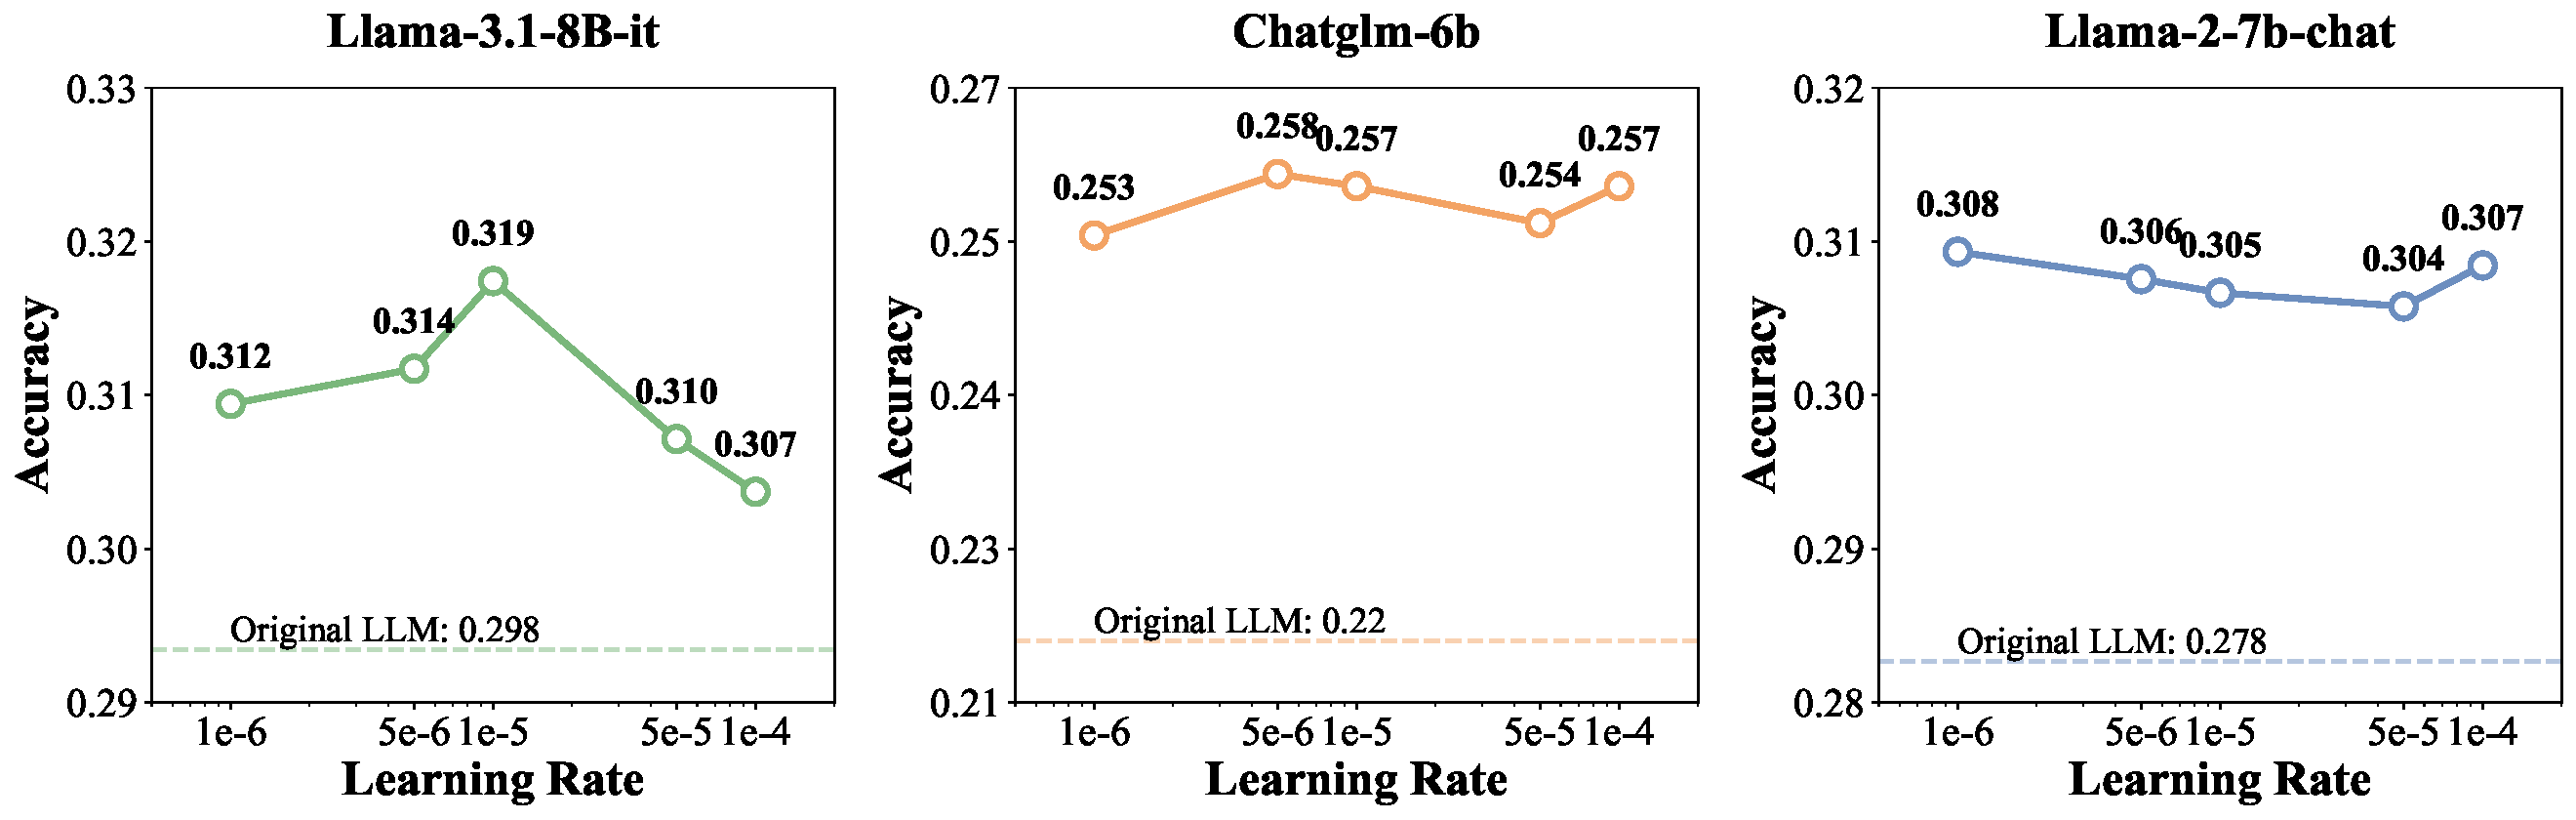
\includegraphics[width=1.0\linewidth]{pic/accuracy_vs_lr.pdf}
  \caption{Accuracy vs. Learning Rate}
  \label{fig:accuracy_vs_lr}
\end{figure}


\begin{figure}[h]
  \centering
  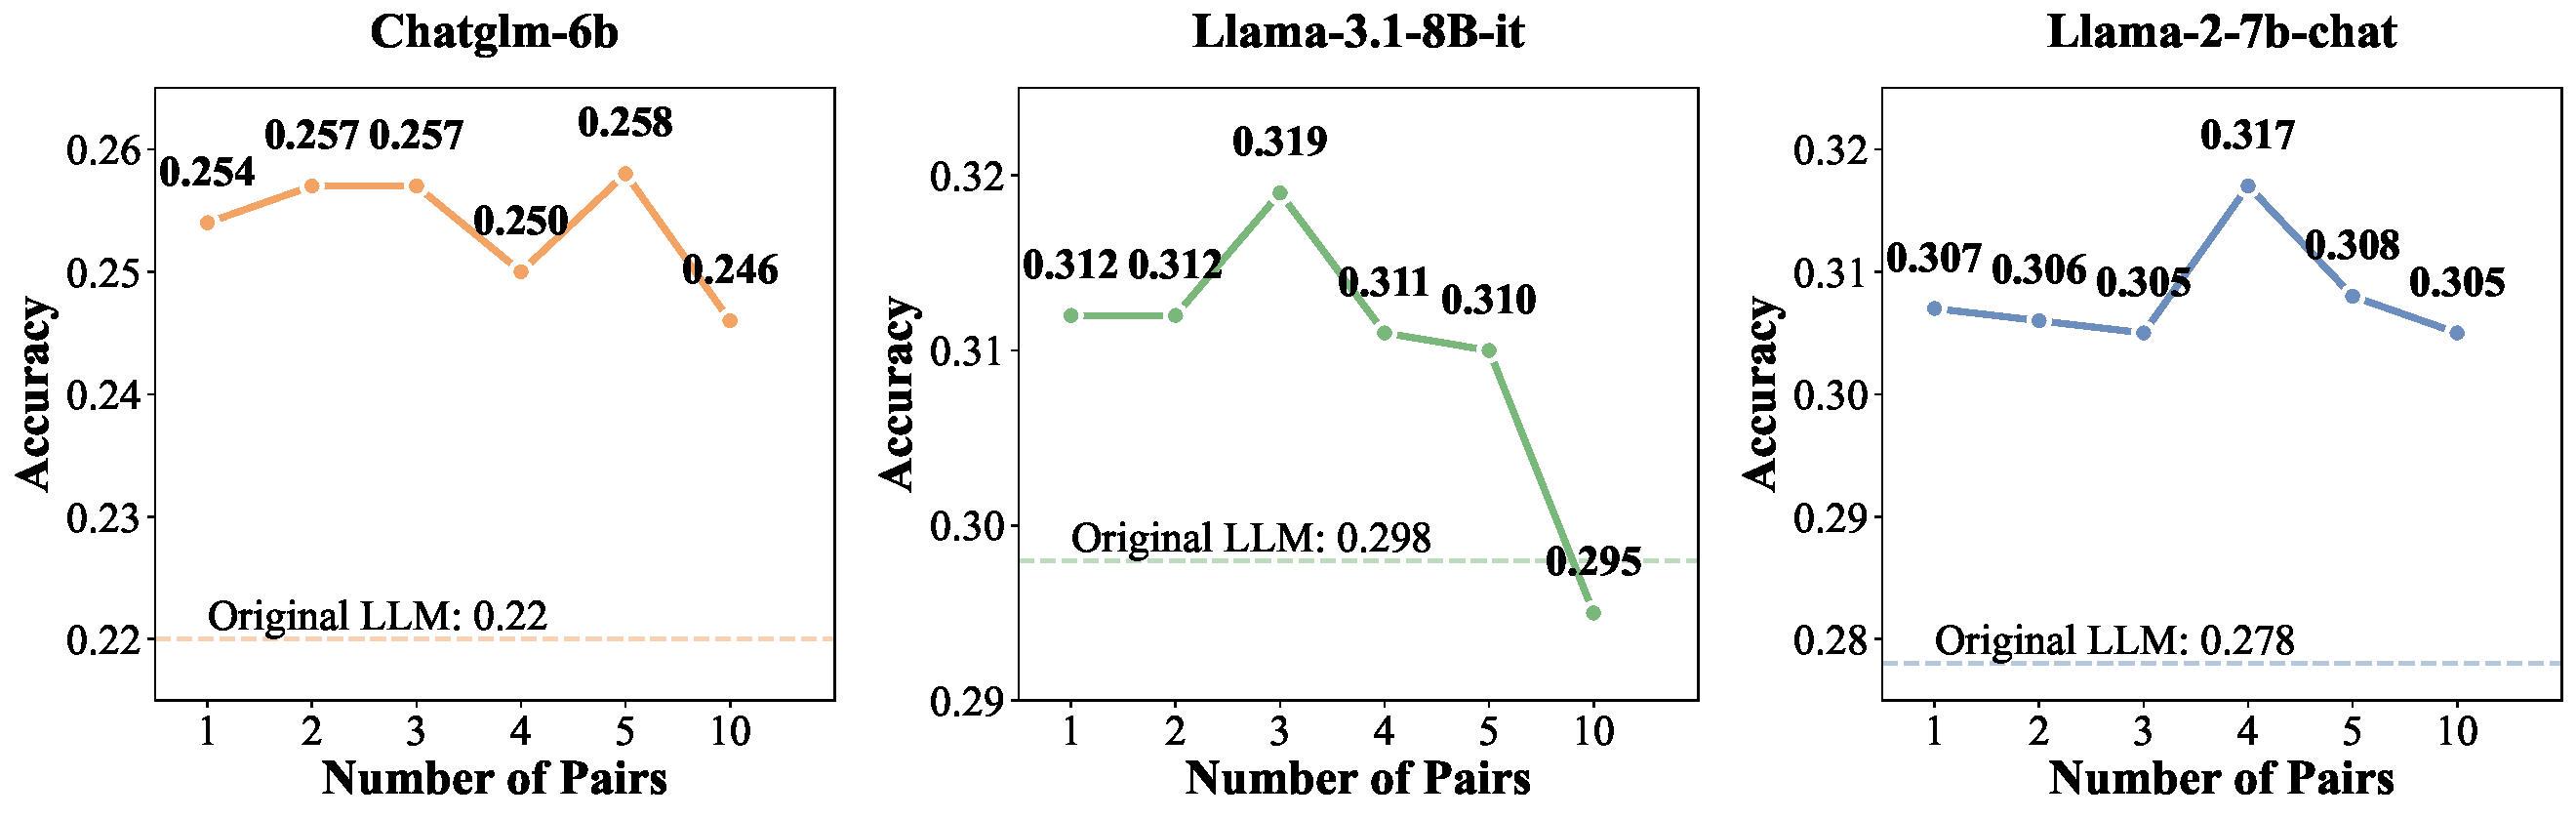
\includegraphics[width=1.0\linewidth]{pic/accuracy_vs_pairs.pdf}
  \caption{Accuracy vs. Number of Adaptation Pairs}
  \label{fig:accuracy_vs_pairs}
\end{figure}

\iffalse
\section{Baseline Details}
\label{appendix:baseline}
We evaluate \ourmethod{} using three state-of-the-art instruction-tuned LLMs: \textbf{Llama-2-7b-chat} \cite{touvron2023llama}, \textbf{Llama-3.1-8b-it} \cite{llama3}, and \textbf{ChatGLM3-6b} \cite{glm2024chatglm}. We compare against two widely adopted baselines:

\paragraph{Chain-of-Thought (CoT)} A prompting technique that guides the model to generate step-by-step reasoning before producing the final answer.

\paragraph{In-Context Learning (ICL)} A method that provides relevant examples in the input prompt to demonstrate the desired task behavior.

We also compare \ourmethod with the three state-of-the-art general domain pretrained RAG models:

\paragraph{Ret-Robust} An approach focused on improving retrieval robustness through strategic passage selection during training. The model learns to discriminate between high-quality and low-quality retrieved content by being trained on a carefully curated mix of passages with different relevance levels.

\paragraph{RAAT} A retrieval-augmented model that introduces a novel noise-aware training strategy. It specifically targets the challenge of distinguishing between helpful and misleading retrieved information by incorporating an adaptive training mechanism that exposes the model to varying types of retrieval noise.

\paragraph{Self-RAG} utilizes instruction
fine-tuning to adaptively retrieve passages based
on the question and determine if the passage contains useful information for answering the question.

\fi

%\subsection{Hyperparameter Analysis}
%\label{sec:hyperparameter_analysis}
\noindent\textbf{Hyperparameter Analysis.}
We also conduct hyper-parameter analysis about the number of adaptation pairs and learning rate. 
As shown in Figure~\ref{fig:accuracy_vs_lr} and Figure~\ref{fig:accuracy_vs_pairs}, our experiments show that learning rates between 1e-6 to 1e-5 provide optimal performance, with 3-5 adaptation pairs yielding the best balance between effectiveness and efficiency. However, the performance of \ourmethod is not sensitive to the number of adaptation pairs and learning rate. In almost all cases, the performance of \ourmethod is better than the naive-rag model.

\iffalse
\paragraph{Learning Rate Analysis} We investigate the sensitivity of our method to different learning rates during test-time adaptation with number of adaptation pairs of 3. As shown in Figure~\ref{fig:accuracy_vs_lr}, we evaluate learning rates ranging from 1e-6 to 1e-4 across all three model architectures. Llama-3.1-8B-it achieves optimal performance at 1e-5 (31.9\% accuracy), with performance gradually declining at higher learning rates. ChatGLM-6B shows more robust behavior across different learning rates, reaching peak performance at 5e-6 to 1e-5 (25.8\% accuracy). Llama-2-7B-chat demonstrates the most stable performance curve, with accuracy varying only slightly (30.4-30.8\%) across all tested learning rates, peaking at 1e-6 (30.8\% accuracy). These results suggest that smaller learning rates (1e-6 to 1e-5) generally provide better and more stable adaptation, likely because they prevent over-aggressive parameter updates that could disrupt the model's pre-trained knowledge. All models show consistent improvement over their original performance (indicated by dashed lines) across most learning rates, validating the robustness of our approach.




\paragraph{Number of Adaptation Passages} We examine how the number of retrieved passages used for adaptation affects performance. This study helps determine the optimal amount of context needed for effective adaptation while considering computational efficiency. As shown in Figure~\ref{fig:accuracy_vs_pairs}, we observe different optimal points across model architectures. Llama-3.1-8B-it achieves peak performance with 3 adaptation pairs (31.7\% accuracy), while Llama-2-7B-chat shows optimal results at 4 pairs (31.7\% accuracy). ChatGLM-6B maintains relatively stable performance between 2-5 pairs, peaking at 5 pairs (25.8\% accuracy). Notably, all models show performance degradation when using 10 pairs. This degradation likely stems from over-aggressive parameter updates that disrupt the model's pre-trained knowledge. Too many adaptation pairs may cause excessive deviation from the original parameters, compromising the valuable knowledge acquired during pre-training. These results indicate that a moderate number of adaptation pairs (3-5) generally provides the best balance between adaptation effectiveness and preserving the model's pre-trained knowledge.
\fi



\noindent\textbf{On the computation efficiency.}
To evaluate the computational overhead of our approach, we measure the total inference time across different configurations and compare it with baseline methods. The computation time reported in Table~\ref{tab:computation} was measured on the CRAG dataset, processing 2,706 queries on one NVIDIA A100 GPU. For each query, up to 5 passages were used for \ourmethod adaptation. Table~\ref{tab:computation} shows the total and average inference times for different numbers of adaptation pairs (1-5), compared against Chain-of-Thought (CoT) and the original model without adaptation. The results are based on processing 2,706 queries from the CRAG dataset.

% TODO: add the average passage length and query length
\begin{table}[h]
\centering
\footnotesize
\caption{Computation time analysis. Total and average inference times (in seconds) for different numbers of adaptation pairs, compared against CoT and vanilla model.}
\label{tab:computation}
\begin{tabular}{@{}l@{\hspace{4pt}}c@{\hspace{4pt}}c@{\hspace{4pt}}c@{\hspace{4pt}}c@{\hspace{4pt}}c@{\hspace{4pt}}c@{\hspace{4pt}}c@{}}
\toprule
\textbf{Metric} & \textbf{1pair} & \textbf{2pair} & \textbf{3pair} & \textbf{4pair} & \textbf{5pair} & \textbf{CoT} & \textbf{Naive-RAG} \\
\midrule
 Total (s) & 4,740 & 5,723 & 6,621 & 7,001 & 7,023 & 11,688 & 961 \\
Avg (s) & 1.75 & 2.11 & 2.45 & 2.59 & 2.60 & 4.32 & 0.36 \\
\bottomrule
\end{tabular}
\end{table}

While our method does introduce additional computational overhead compared to the original model, it remains significantly more efficient than CoT. The average processing time per query ranges from 1.75s (1-pair) to 2.60s (5-pair), which is substantially lower than CoT's 4.32s. This demonstrates that \ourmethod achieves its performance improvements with reasonable computational cost, making it practical for real-world applications.

\section{Conclusion}

In this paper, we present \ourmethod, a test-time adaptation approach for retrieval-augmented generation that enables dynamic model optimization during inference. Our method introduces a simple yet effective self-supervised learning objective where the model learns to predict retrieved content, allowing automatic parameter adjustment to target domains without requiring labeled data. Through extensive experiments across six specialized domain, we demonstrate that \ourmethod achieves consistent improvements over the naive-rag system. These findings suggest that test-time adaptation is a promising direction for improving RAG systems' performance in specialized domains.


\iffalse
\section*{Limitations}
While \ourmethod demonstrates promising performance improvements, several limitations and areas for future work should be acknowledged.

First, the test-time adaptation process, although lightweight compared to methods like Chain-of-Thought for a small number of adaptation pairs, still introduces computational overhead during inference. As shown in our experiments (Table~\ref{tab:computation}), adapting on 5 pairs adds approximately 2.24 seconds per query compared to the vanilla model (0.36s vs 2.60s). This additional latency might be a concern for highly latency-sensitive applications. Furthermore, the process involves gradient updates and optimizer state management, which increases GPU memory consumption during inference compared to standard RAG systems. This could pose challenges for deployment on resource-constrained devices or with very large models.

Second, the current strategy involves resetting model parameters to their original pre-trained state before adapting to each new query. While this ensures that adaptation for one query does not detrimentally affect the next, it does mean that computations for adaptation are repeated for each query. This leads to a higher overall computational load and could be considered less environmentally friendly due to the repeated computations. Future research could explore strategies for more persistent or incremental adaptation that carry over some learned adaptations without catastrophic forgetting or negative interference between queries.

Third, the scalability of \ourmethod when faced with a very large number of retrieved passages per query (e.g., dozens or hundreds, as some systems might retrieve) has not been fully explored. Our current experiments adapt on a small number (1-5) of passages. Adapting on a significantly larger set would proportionally increase the computational overhead. Strategies for intelligently selecting a subset of the most informative passages for adaptation, or more efficient batched adaptation techniques, would be necessary in such scenarios.

Fourth, while our empirical results are strong, the paper provides a more intuitive rather than a deeply theoretical justification for the prefix-suffix adaptation strategy. A more formal analysis of why this specific self-supervised task is effective for domain adaptation in RAG, perhaps compared to other potential self-supervised objectives, could further strengthen the approach.

Finally, our experiments primarily focused on models up to 8 billion parameters. Investigating the applicability and effectiveness of \ourmethod on a wider range of model sizes, including smaller models (e.g., 1.5B, 3B) and significantly larger ones (e.g., 70B+), would provide a more comprehensive understanding of its generalizability.

Addressing these limitations could enhance the practicality and applicability of test-time adaptation for RAG systems in diverse real-world scenarios.
\fi

% \section*{Ethical Considerations}
% Test-time adaptation may potentially affect the model's safety alignment due to parameter updates. However, since our method only updates parameters for a limited number of iterations, the model's safety alignment likely remains largely intact, with minimal risk of disruption. Nevertheless, we believe it is important to investigate the extent to which gradient updates on domain-specific data can impact a model's established safety alignment without compromising it. This represents an important direction for future research to better understand the relationship between adaptation and safety preservation.

%%
%% The next two lines define the bibliography style to be used, and
%% the bibliography file.






\iffalse
\section{Implementation Details}
We use Llama-3.1-8b-instruct, ChatGLM-3-6b, Llama-2-7b-chat as our backbone models.  Here we detail the hyperparameters and configuration settings used in our implementation. For the optimization process, we employ a learning rate of 1e-5, which provides a balance between adaptation effectiveness and stability. To improve training efficiency while managing memory constraints, we implement gradient accumulation with 2 steps. Gradient clipping is set at 0.1 to prevent gradient explosions, particularly important during rapid adaptation to new contexts. We use the AdamW optimizer with weight decay of 0.01 and epsilon of 1e-8, which helps prevent overfitting while maintaining numerical stability. Additional controls include filtering out sentences shorter than 6 tokens and limiting adaptation to 3 pairs per step. These parameters were determined through extensive experimentation across various domains, optimizing for both adaptation performance and computational efficiency. All experiments were conducted three times and the average results are reported.

All experiments are conducted on NVIDIA A100 GPUs with 80GB of memory. We utilize a fixed random seed of 42, and the experimental results are reported within a single run. For implementation, we use the following library versions: transformers 4.30.2, torch 2.1.0.
\fi


    

\iffalse
\section{Licensing}
The CRAG, BioASQ and PubMedQA datasets are released for academic usage. These datasets are designed for evaluating RAG systems. Thus, our use of these datasets is consistent with their intended use.

The language models used in our experiments are released under the following licenses: \textbf{Llama-2-7b-chat} \cite{touvron2023llama} is released under the Meta Llama 2 Community License Agreement. It is a variant of the Llama 2 family released in July 2023, featuring 7 billion parameters and specifically optimized for dialogue applications. \textbf{Llama-3.1-8b-it} \cite{llama3} is released under the Llama 3 License. Released in April 2024, it features 8 billion parameters and is specifically designed for instruction-following tasks, representing one of the most advanced open-source LLMs. \textbf{ChatGLM3-6b} \cite{glm2024chatglm} is released under the Apache 2.0 License. It is a bilingual conversational language model featuring 6 billion parameters, demonstrating strong performance in both English and Chinese tasks.  All these models are open for academic usage.
\fi



%%
%% If your work has an appendix, this is the place to put it.
% \appendix
\footnotesize
\bibliographystyle{IEEEbib}
\bibliography{custom, anthology}

\end{document}
